\section{Observation-Level Transfer}
Observation-level \simtoreal focuses on aligning perception between sim and reality. The dominant strategy is \emph{visual domain randomization}, which artificially varies rendering during training (textures, lighting, colors, camera pose) so that the policy learns invariant features \cite{Sadeghi2017,Tobin2017}. For example, Sadeghi and Levine’s CAD2RL rendered randomized indoor scenes for a quadrotor, enabling a monocular vision policy to generalize to real hallways (without any real images for training)\cite{Sadeghi2017}. Figure~\ref{fig:adr_pipeline}(A) illustrates how ADR similarly randomizes environments (OpenAI Rubik’s Cube example): the learned vision encoder and policy must cope with varied camera views and object appearances. Domain randomization is popular because it requires no real data and often suffices if the randomized range covers the real-world variability. However, it can lead to inefficiency or failure if unrealistic combinations are included or if the real domain lies outside the chosen randomization range.

Beyond randomization, \emph{domain adaptation} methods use learning to map between sim and real observations. For example, generative techniques (e.g.\ CycleGAN or SimGAN) can transform real camera images into the simulator’s style, or vice versa, and then apply a sim-trained policy\cite{Tzeng2017}. These methods may require some real data or paired images, which partially defeats the pure sim-training advantage. In practice, adaptation is more common in perception (e.g.\ object detection) than in end-to-end RL due to the difficulty of adversarial training in policy learning.

Another approach is \emph{sensor modeling and augmentation}: simulating sensor noise, delays, or partial observability in training. For example, adding realistic noise to depth or lidar readings, or dropping out camera pixels, can make a learned policy robust to sensor imperfections. Similarly, using multi-modal inputs (e.g.\ combining vision and proprioception) can reduce reliance on any single sim-only signal. Some works design a compact observation space to eliminate noisy dimensions: Tan et al.\ found that excluding the robot’s yaw angle (which drifted) improved transfer for quadruped control\cite{Tan2018}. 

Overall, observation-level transfer is well-served by domain randomization and careful sensor simulation. These methods, combined with powerful neural encoders, allow policies to generalize across texture and lighting variations\cite{Tobin2017,Sadeghi2017}. Figure~\ref{fig:adr_pipeline}(A) illustrates this concept: the vision system is trained on many randomized versions of the cube and hand. We will use Fig.~\ref{fig:adr_pipeline} again below to show how those observations feed into the policy and state estimator.

\begin{figure}[H]
    \centering
    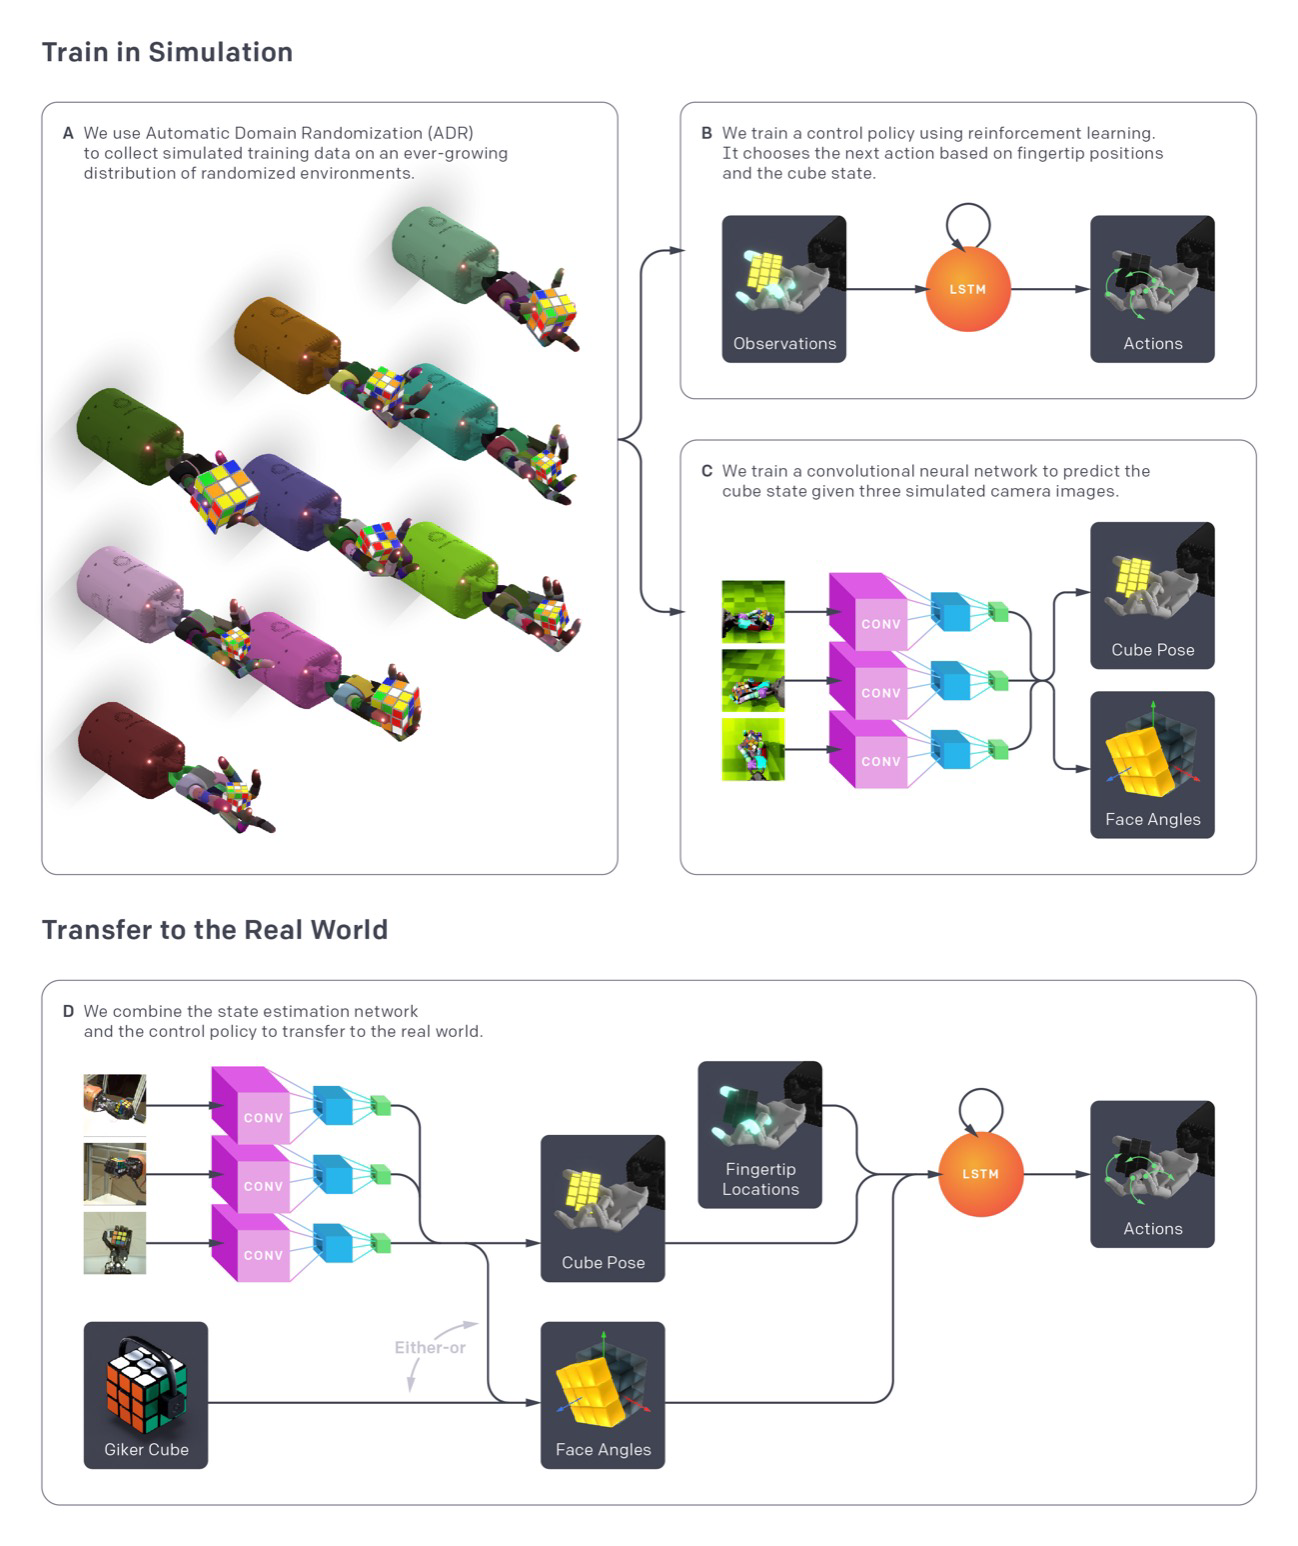
\includegraphics[width=0.95\linewidth]{figures/figAdrPipeline.png}
    \caption{Training pipeline with Automatic Domain Randomization (ADR) for \simtoreal transfer. (A) Simulation generates randomized cube-and-hand images; (B) a policy (LSTM) maps simulated observations (hand and cube states) to actions; (C) a CNN state estimator is trained to predict cube pose from images; (D) during real-world deployment, camera images pass through the CNN, then policy acts on estimated state. (\emph{Adapted from} Akkaya et al.~\cite{Akkaya2019}.)}
    \label{fig:adr_pipeline}
\end{figure}

\paragraph{Evaluation.} Domain randomization for visual perception has shown robust performance in tasks such as drone navigation (CAD2RL~\cite{Sadeghi2017}) and robotic manipulation (Dactyl~\cite{Akkaya2019}). Its main advantage is that it requires no real-world data and can be scaled easily. However, its effectiveness is sensitive to the diversity and realism of the randomized features. Over-randomization or unrealistic textures can degrade learning efficiency. Domain adaptation methods offer finer alignment but typically require real data and are challenging to scale to end-to-end RL pipelines~\cite{Tzeng2017}.
